
\subsection{Трехмерная задача просачивания в резервуаре с источником на границе}

Рассмотрим трехмерную область пористой среды, имеющую форму
куба, верхняя поверхность открытая, нижняя грань ограничена резервуаром, через боковые грани
может происходить просачивание.
В начальный момент времени водой занято лишь
10\% области, а для нефти и газа задано периодическое распределение. Ось $y$ направлена снизу-вверх.
На верхней грани в углу, расположен источник воды, он занимает девятую часть поверхности.
Месторасположение источника нагревается.
Просачивание происходит под действием силы тяжести. 
Для ускорения процесса просачивания значение ускорения свободного падения положено равным 98 $\text{м/с}^2$.
Пусть число расчетных узлов -- $N_x\cdot N_y\cdot N_z$.\\
Начальные условия:
\begin{equation}
  \begin{aligned}
    &S_w=0.1,\\
    &S_n(x, y, z)=0.4 + 0.1 \cdot sin^2(x \cdot N_x + y \cdot N_y + z \cdot N_z),\\
    &S_g(x, y, z)=0.4 + 0.1 \cdot cos^2(x \cdot N_x + y \cdot N_y + z \cdot N_z),\\
    &P_w=P_\text{атм},\\
    &T=285K.
   \end{aligned}
\end{equation}
Граничные условия:
\begin{equation}
  \begin{aligned}
    &\left.T\right|_{y=1,\ 0 < x < 0.33,\ 0 < z < 0.33}=320K,\\
    &\left.P\right|_{y=1,\ 0 < x < 0.33,\ 0 < z < 0.33}=P_{\text{атм}},\\
    &\left.{P_i}\right|_{y=0}\text{ определяется из условия } \left.(\overrightarrow{u_i} \cdot \overrightarrow{n})\right|_{y=0}=0;\\
    &\left.S_w\right|_{y=1,\ 0 < x < 0.33,\ 0 < z < 0.33}=0.6,\\
    &\left.S_n\right|_{y=1,\ 0 < x < 0.33,\ 0 < z < 0.33}=0.05,\\
    &\text{на остальных граничных поверхностях потоки}\\
    &T,\ S_w,\ S_n,\ P_w\ \text{через нормаль равны нулю.}
  \end{aligned}
\end{equation}

Результаты расчетов изображены на Рис.~\ref{t4_pic_start} - Рис.~\ref{t4_pic_end}, приведены распределения давления, температуры
и~ насыщенностей трех фаз в три различные момента времени. Можно видеть, что фронты источника распространяются по
области, около нижней границы происходит накопление воды, вода постепенно вытесняет нефть и газ через боковые и верхнюю грани.

\begin{figure}
  \begin{center}
    \begin{minipage}[h]{0.49\textwidth}
       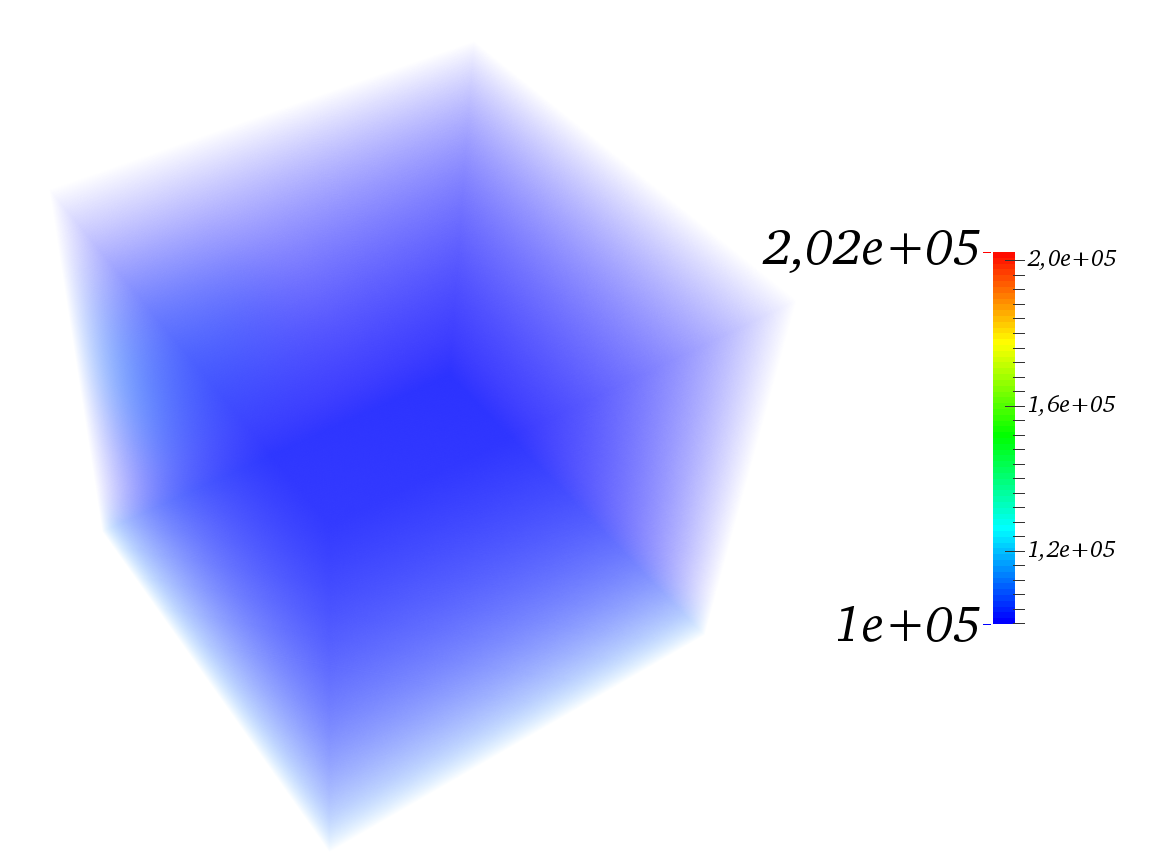
\includegraphics[width=1\textwidth]{test4/pw_200.png}
       \vspace{1cm}
       \caption{Давление $P_w$ в момент времени $t=200$с}
       \label{t4_pic_start}
    \end{minipage}
    \hfill
    \begin{minipage}[h]{0.49\textwidth}
       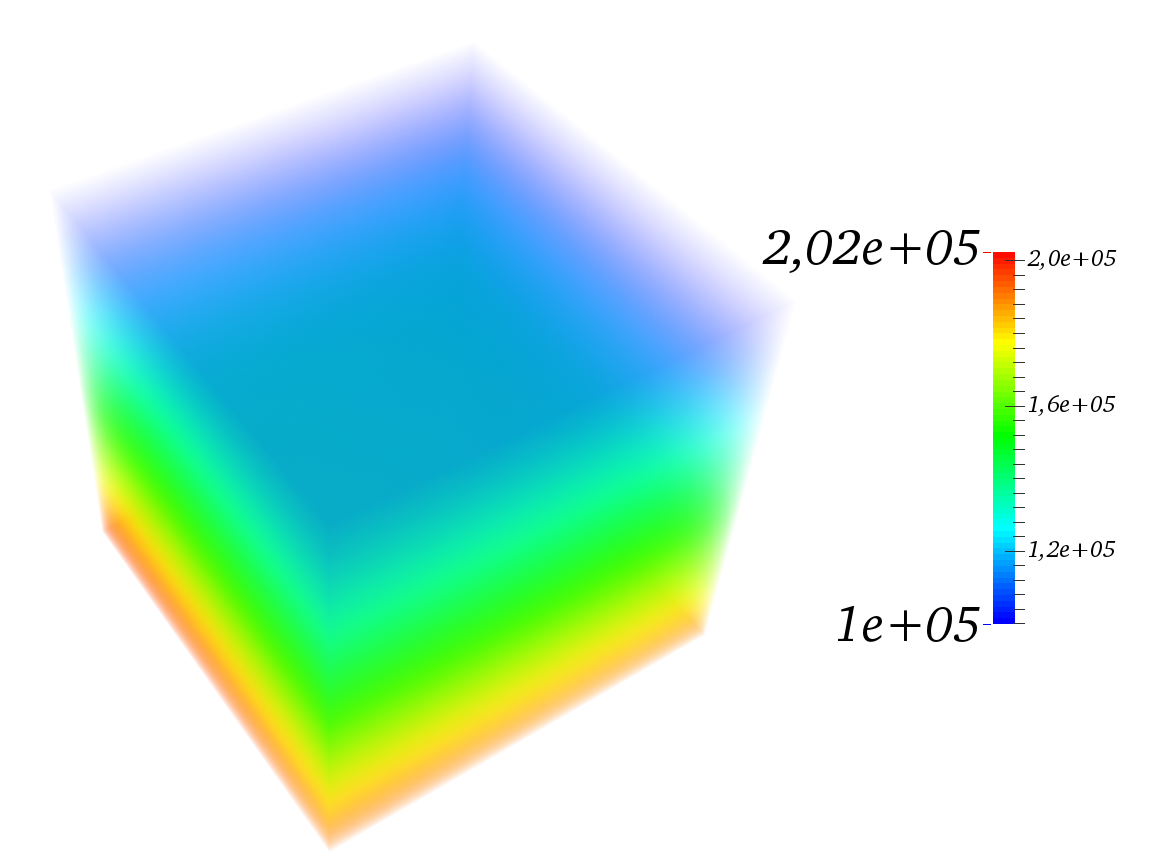
\includegraphics[width=1\textwidth]{test4/pw_1000.png}
       \vspace{1cm}
       \caption{Давление $P_w$ в момент времени $t=1000$с}
    \end{minipage}
    \vspace{3cm}
    \vfill
    \begin{minipage}[h]{0.49\textwidth}
       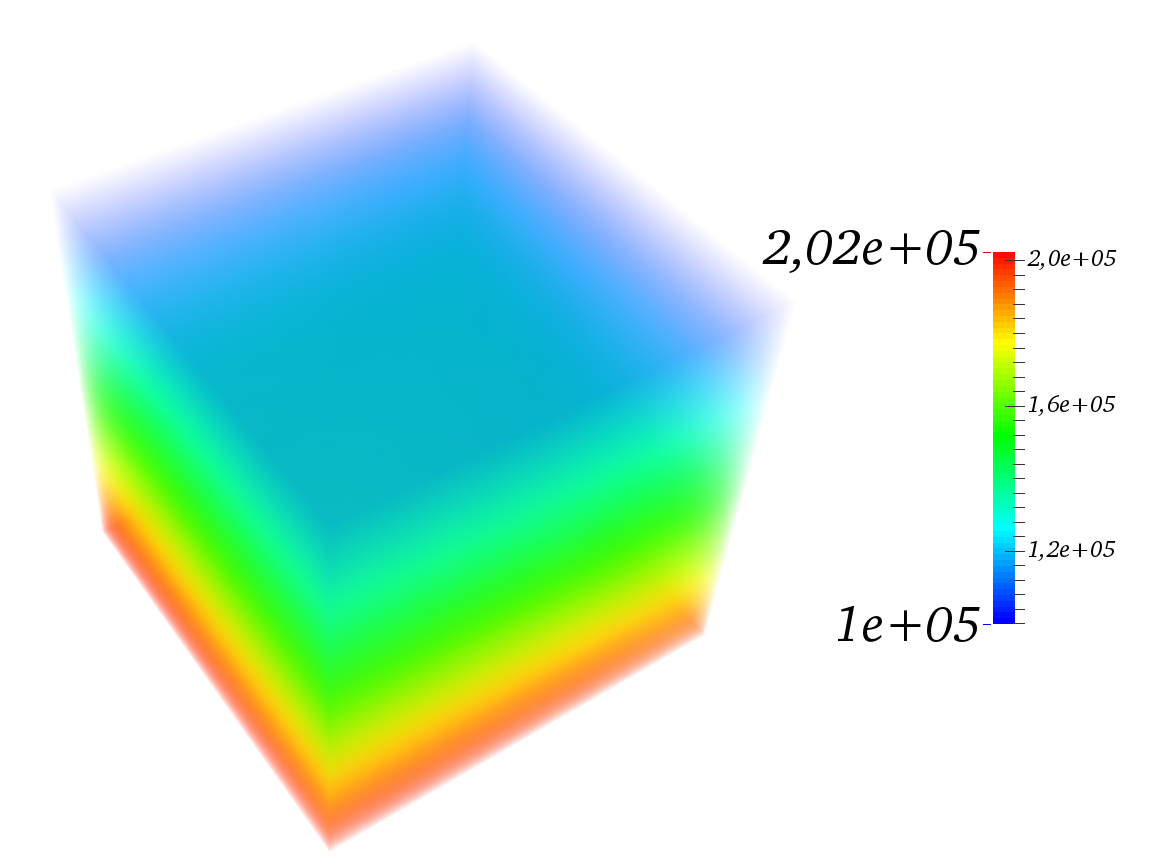
\includegraphics[width=1\textwidth]{test4/pw_2000.png}
       \vspace{1cm}
       \caption{Давление $P_w$ в момент времени $t=2000$с}
    \end{minipage}
    \hfill
    \begin{minipage}[h]{0.49\textwidth}
       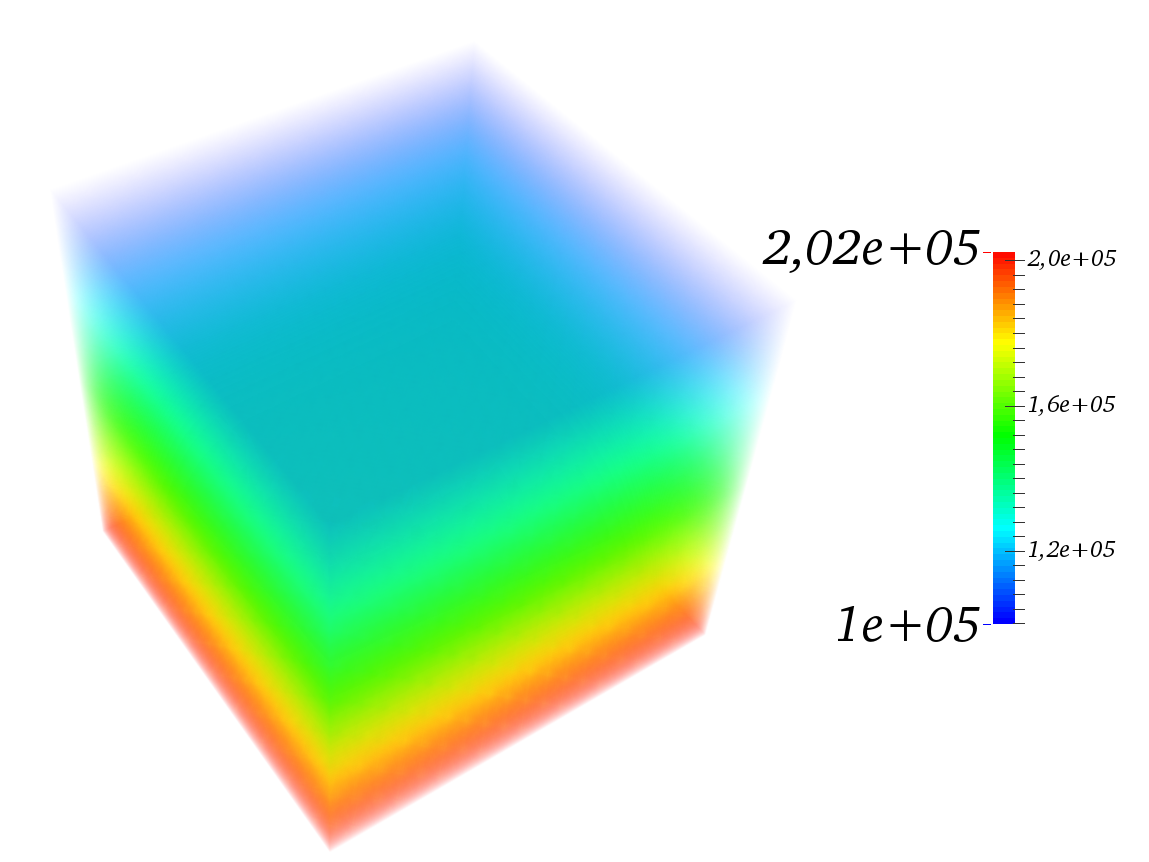
\includegraphics[width=1\textwidth]{test4/pw_6600.png}
       \vspace{1cm}
       \caption{Давление $P_w$ в момент времени $t=6600$с}
    \end{minipage}
    \hfill  
  \end{center}
\end{figure}

\begin{figure}
  \begin{center}
    \begin{minipage}[h]{0.49\textwidth}
       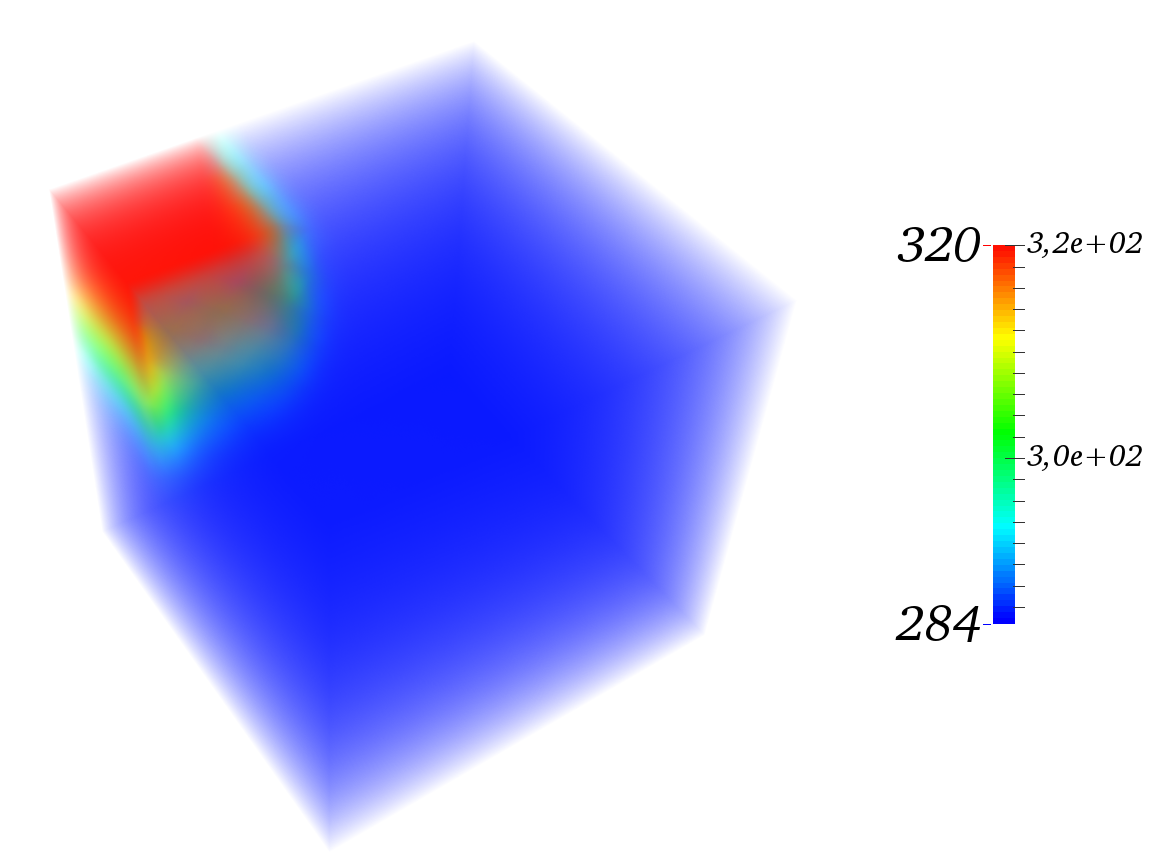
\includegraphics[width=1\textwidth]{test4/t_200.png}
       \vspace{1cm}
       \caption{Температура в момент времени $t=200$с}
    \end{minipage}
    \hfill
    \begin{minipage}[h]{0.49\textwidth}
       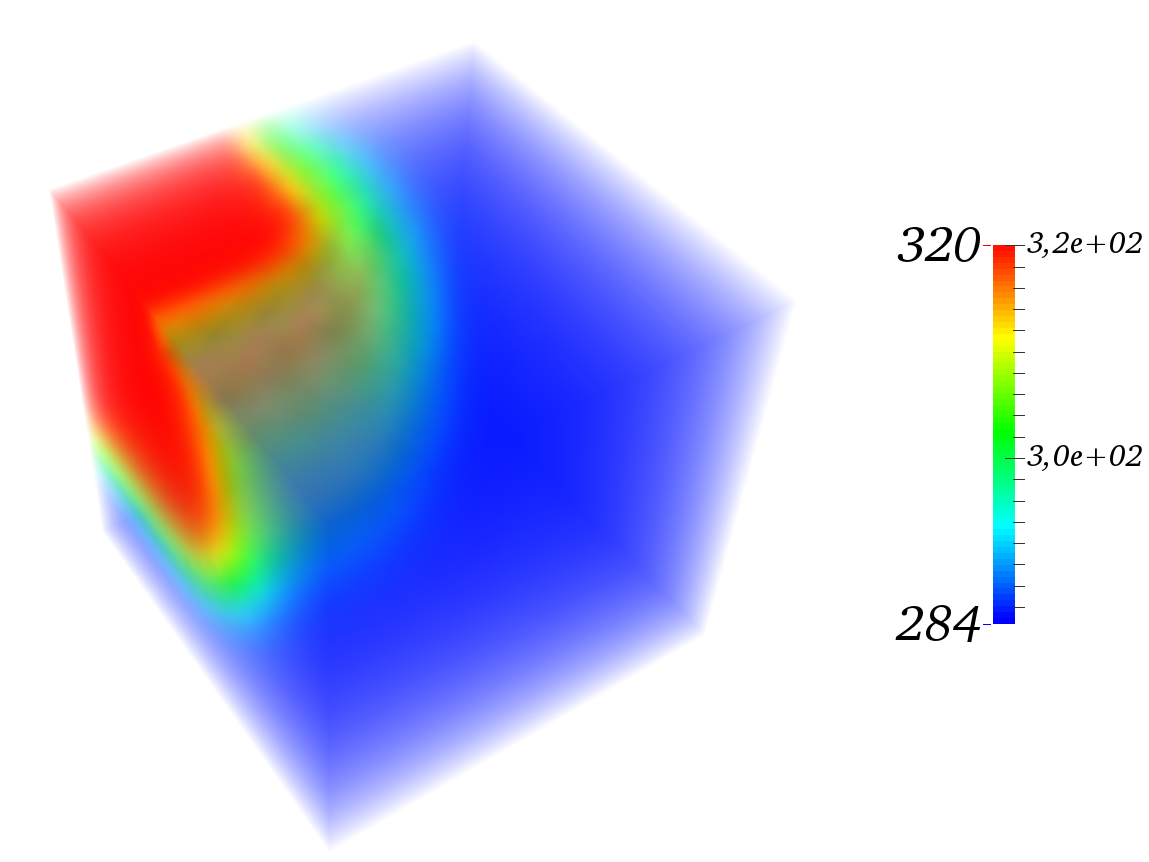
\includegraphics[width=1\textwidth]{test4/t_1000.png}
       \vspace{1cm}
       \caption{Температура в момент времени $t=1000$с}
    \end{minipage}
    \vspace{3cm}
    \vfill
    \begin{minipage}[h]{0.49\textwidth}
       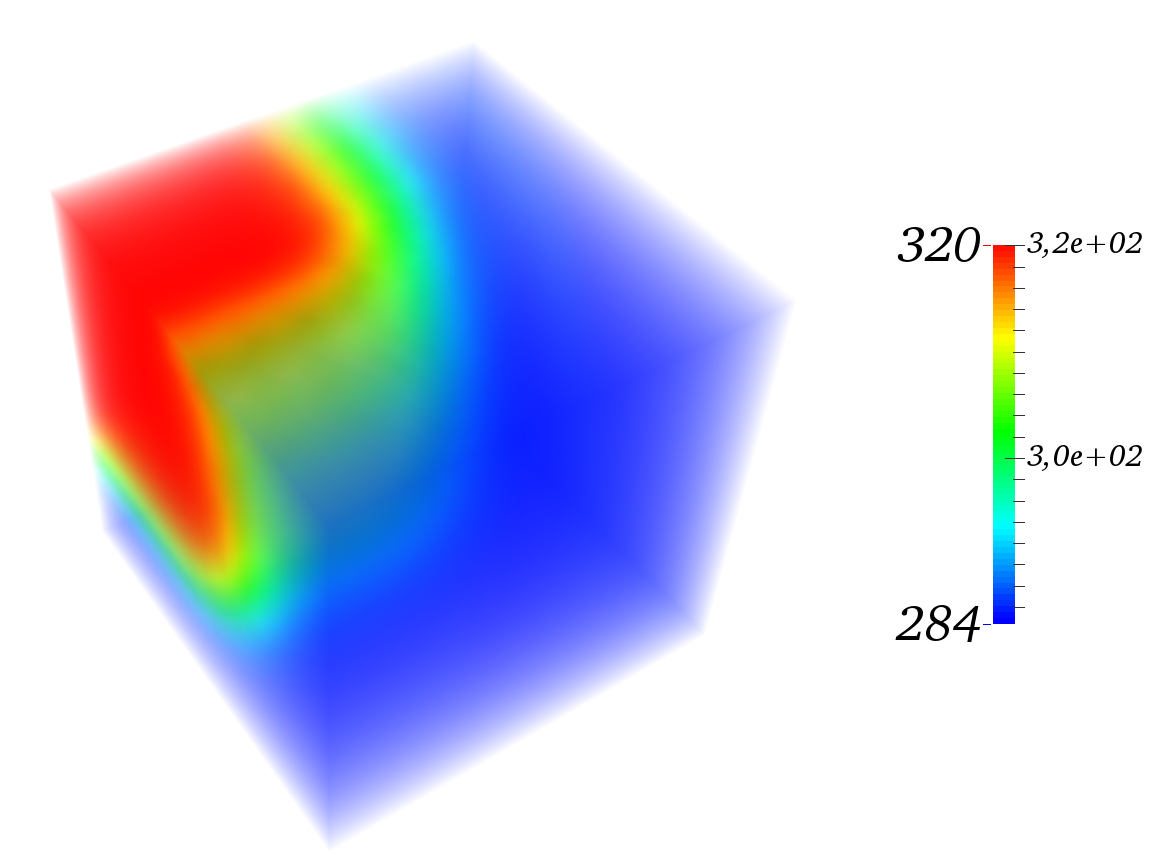
\includegraphics[width=1\textwidth]{test4/t_2000.png}
       \vspace{1cm}
       \caption{Температура в момент времени $t=2000$с}
    \end{minipage}
    \hfill
    \begin{minipage}[h]{0.49\textwidth}
       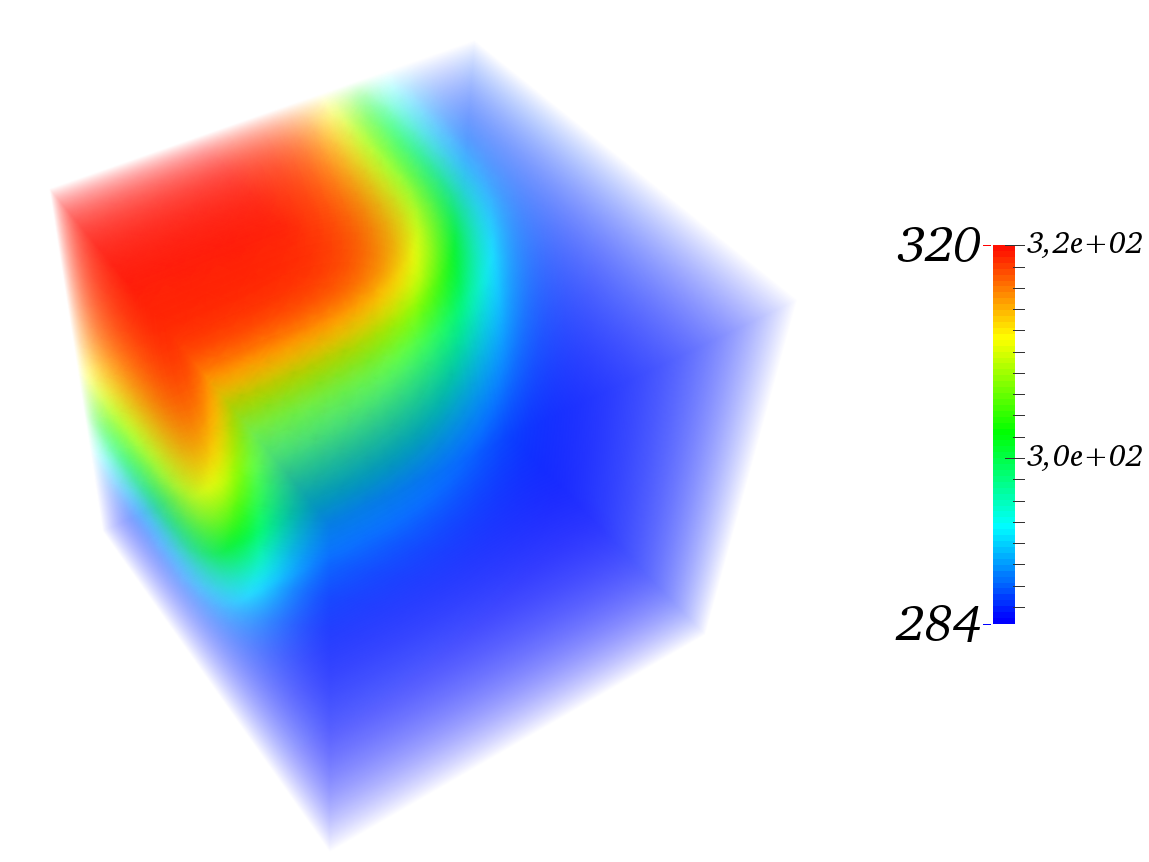
\includegraphics[width=1\textwidth]{test4/t_6600.png}
       \vspace{1cm}
       \caption{Температура в момент времени $t=6600$с}
    \end{minipage}
    \hfill  
  \end{center}
\end{figure}

\begin{figure}
  \begin{center}
    \begin{minipage}[h]{0.49\textwidth}
       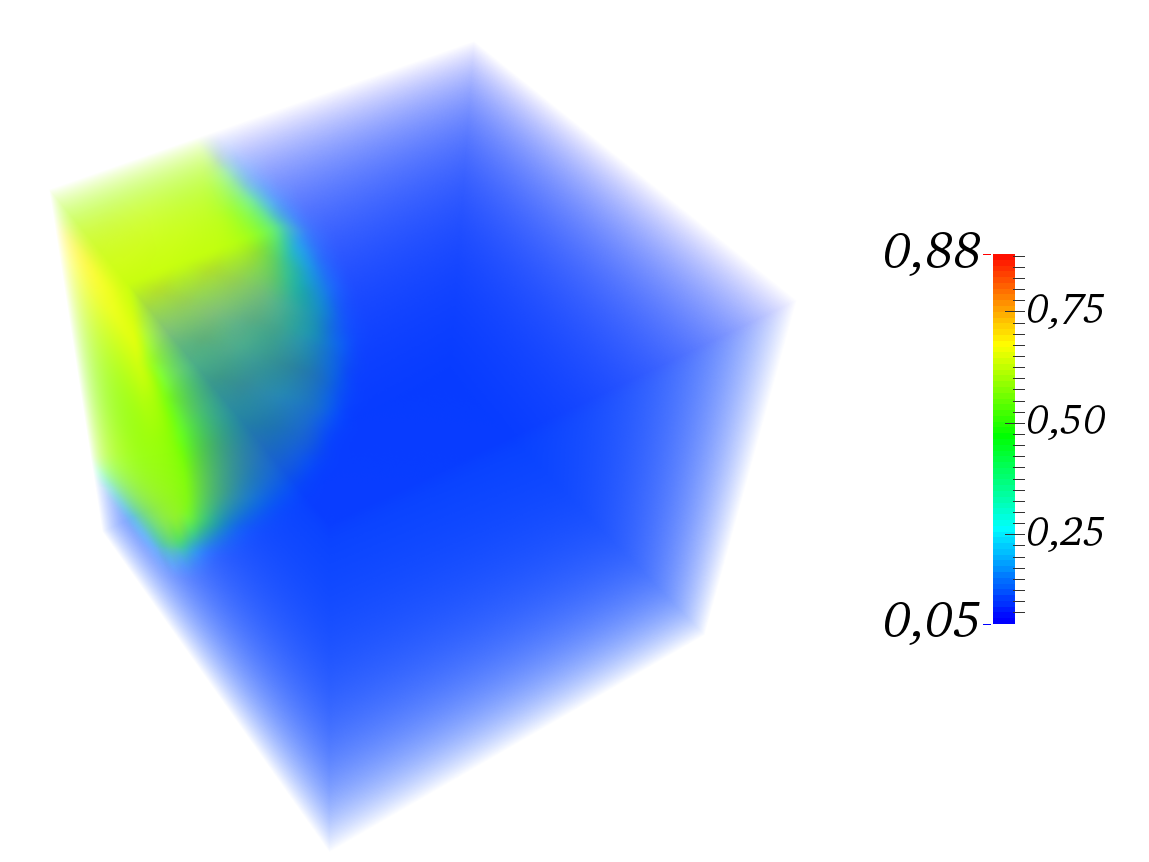
\includegraphics[width=1\textwidth]{test4/sw_200.png}
       \vspace{1cm}
       \caption{Насыщенность $S_w$ в момент времени $t=200$с}
    \end{minipage}
    \hfill
    \begin{minipage}[h]{0.49\textwidth}
       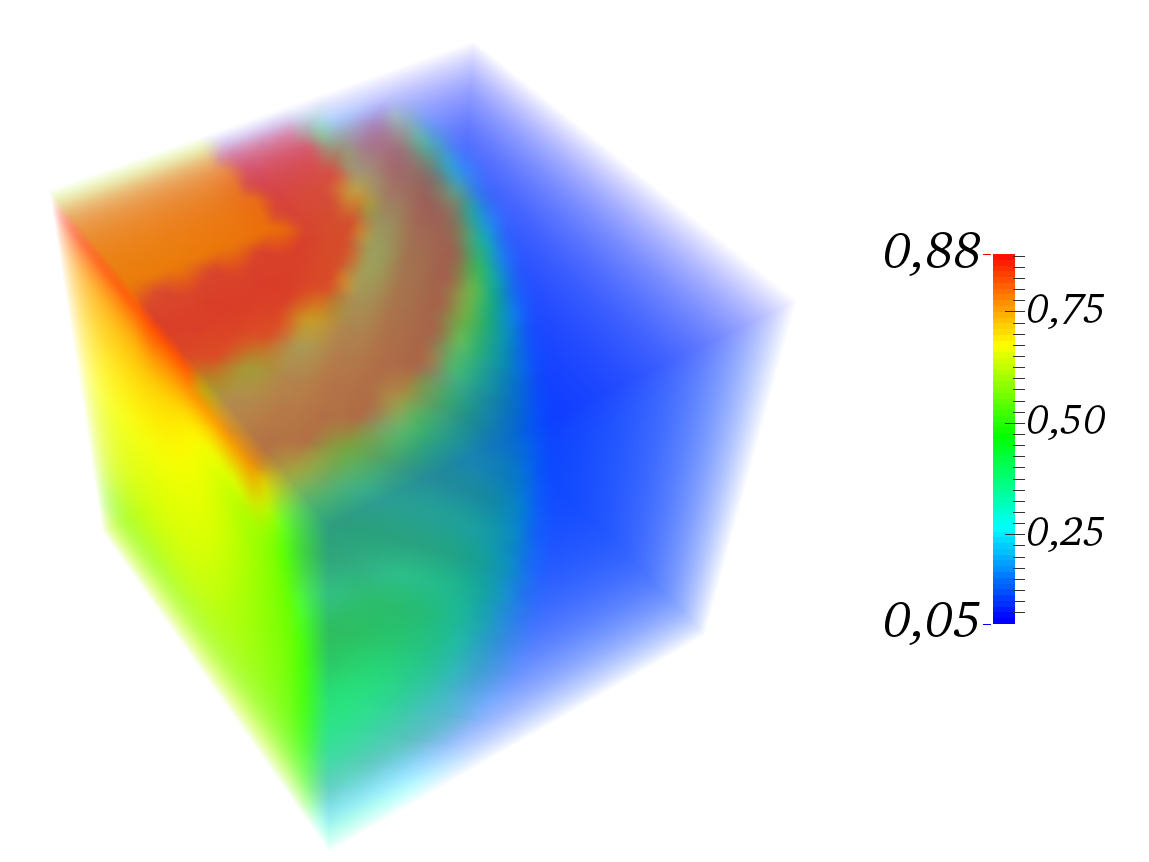
\includegraphics[width=1\textwidth]{test4/sw_1000.png}
       \vspace{1cm}
       \caption{Насыщенность $S_w$ в момент времени $t=1000$с}
    \end{minipage}
    \vspace{3cm}
    \vfill
    \begin{minipage}[h]{0.49\textwidth}
       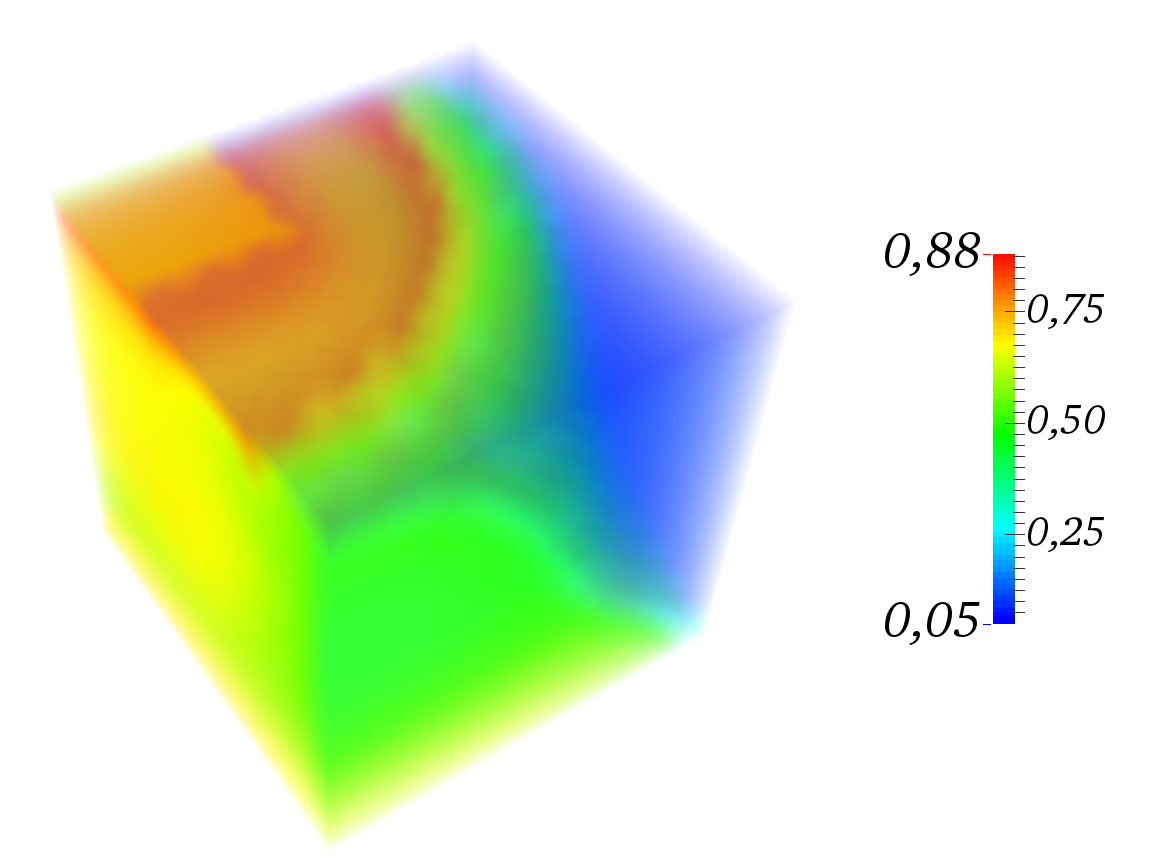
\includegraphics[width=1\textwidth]{test4/sw_2000.png}
       \vspace{1cm}
       \caption{Насыщенность $S_w$ в момент времени $t=2000$с}
    \end{minipage}
    \hfill
    \begin{minipage}[h]{0.49\textwidth}
       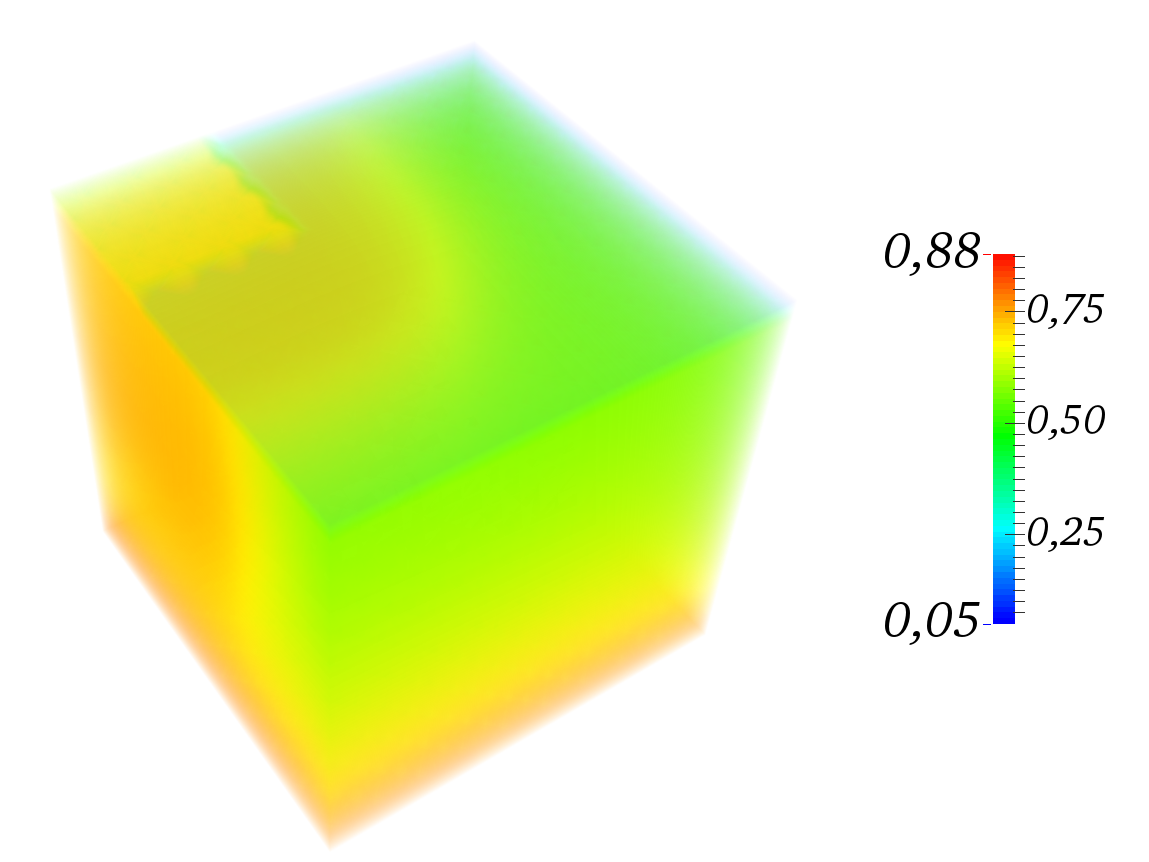
\includegraphics[width=1\textwidth]{test4/sw_6600.png}
       \vspace{1cm}
       \caption{Насыщенность $S_w$ в момент времени $t=6600$с}
    \end{minipage}
    \hfill  
  \end{center}
\end{figure}

\begin{figure}
  \begin{center}
    \begin{minipage}[h]{0.49\textwidth}
       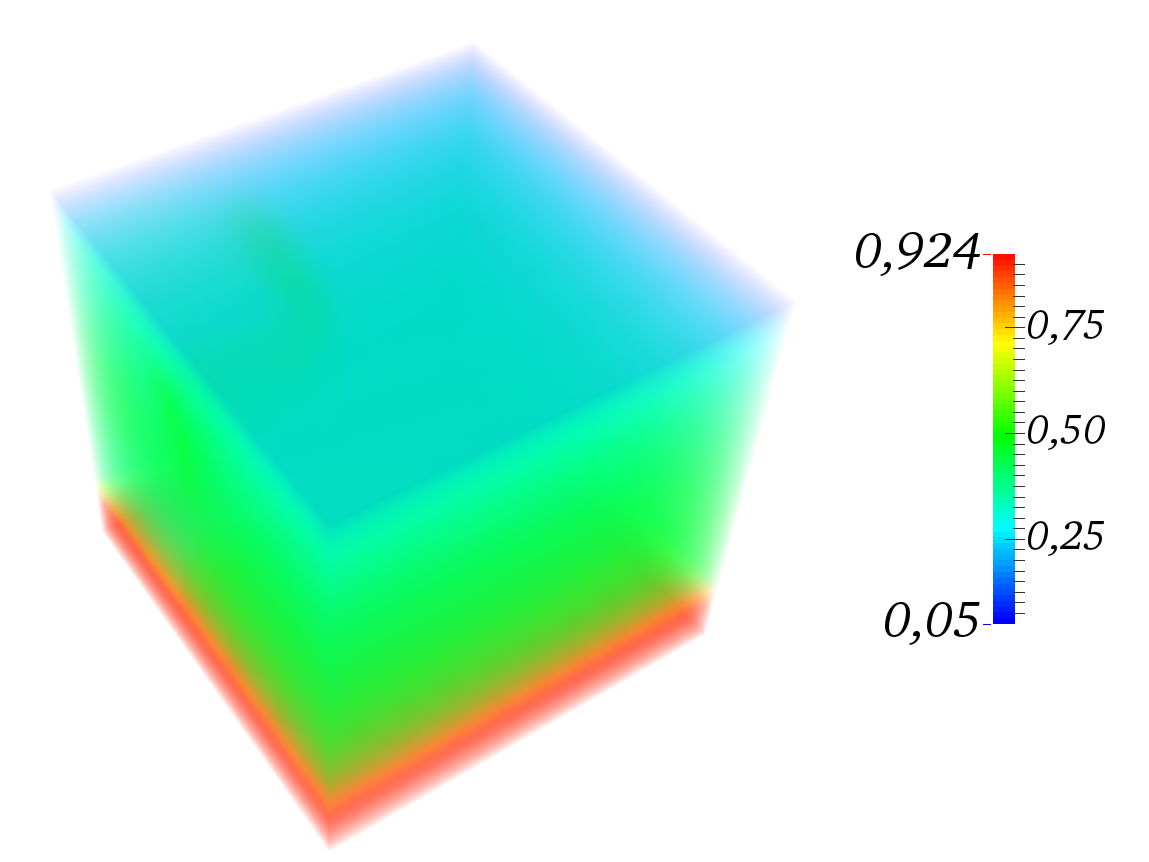
\includegraphics[width=1\textwidth]{test4/sn_200.png}
       \vspace{1cm}
       \caption{Насыщенность $S_n$ в момент времени $t=200$с}
    \end{minipage}
    \hfill
    \begin{minipage}[h]{0.49\textwidth}
       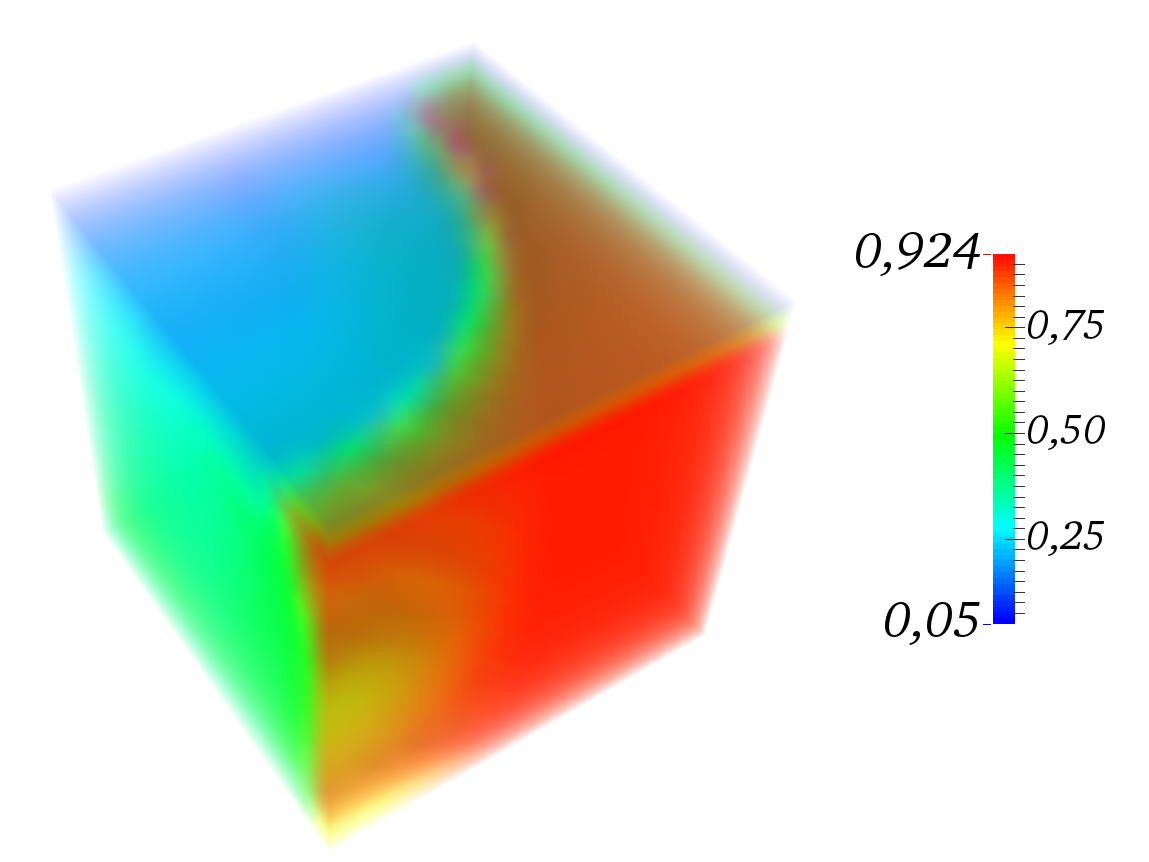
\includegraphics[width=1\textwidth]{test4/sn_1000.png}
       \vspace{1cm}
       \caption{Насыщенность $S_n$ в момент времени $t=1000$с}
    \end{minipage}
    \vspace{3cm}
    \vfill
    \begin{minipage}[h]{0.49\textwidth}
       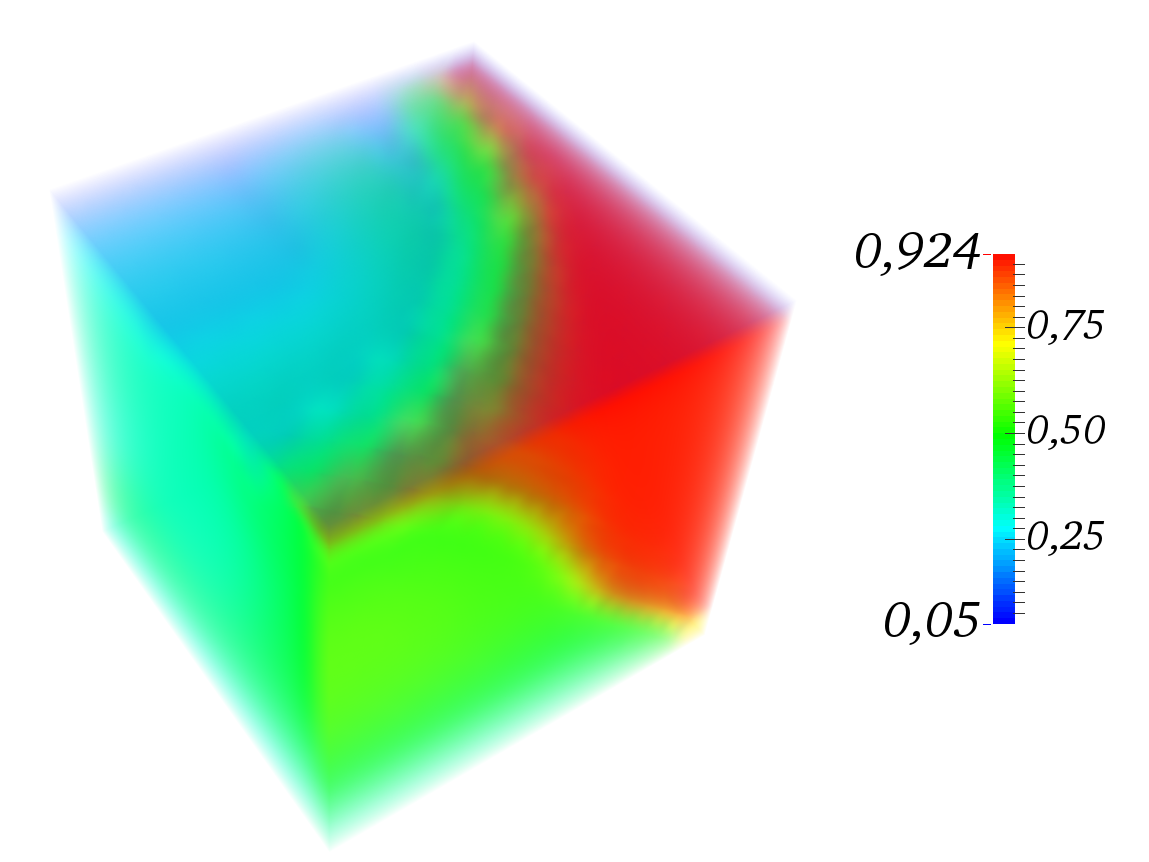
\includegraphics[width=1\textwidth]{test4/sn_2000.png}
       \vspace{1cm}
       \caption{Насыщенность $S_n$ в момент времени $t=2000$с}
    \end{minipage}
    \hfill
    \begin{minipage}[h]{0.49\textwidth}
       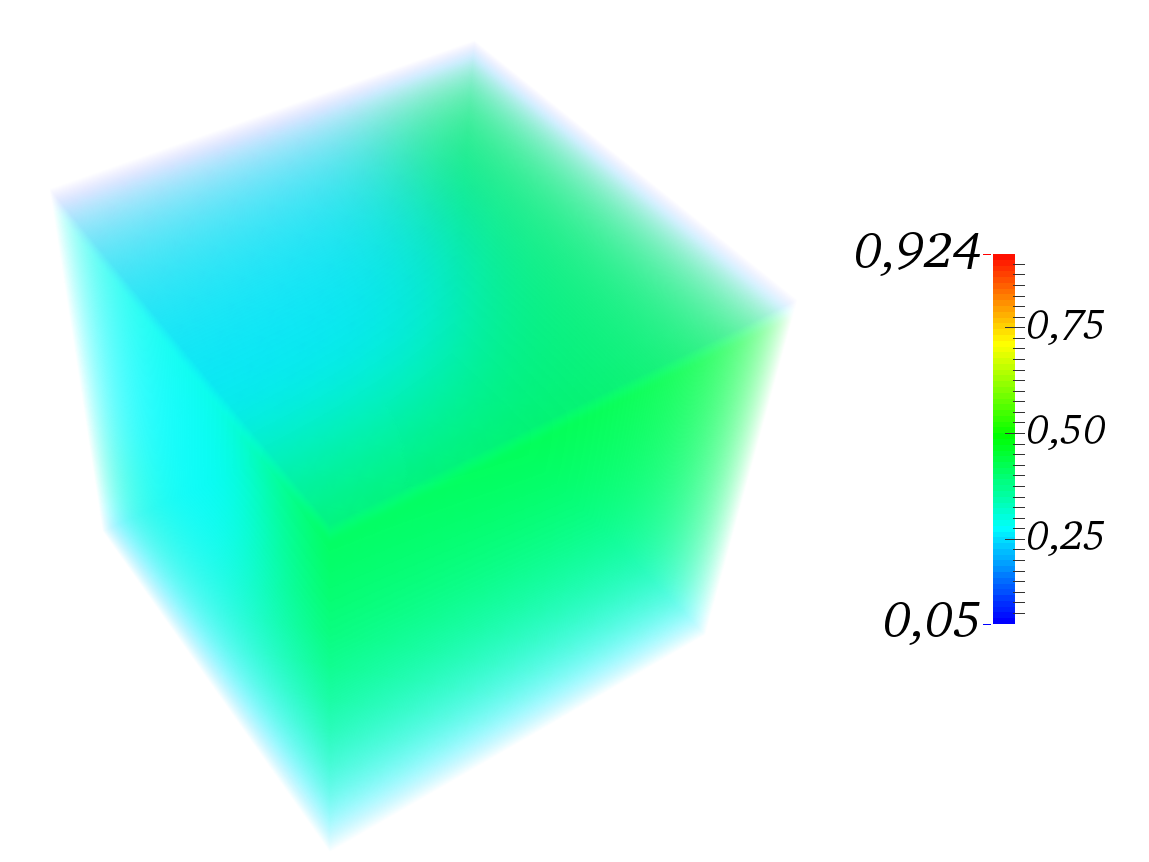
\includegraphics[width=1\textwidth]{test4/sn_6600.png}
       \vspace{1cm}
       \caption{Насыщенность $S_n$ в момент времени $t=6600$с}
    \end{minipage}
    \hfill  
  \end{center}
\end{figure}

\begin{figure}
  \begin{center}
    \begin{minipage}[h]{0.49\textwidth}
       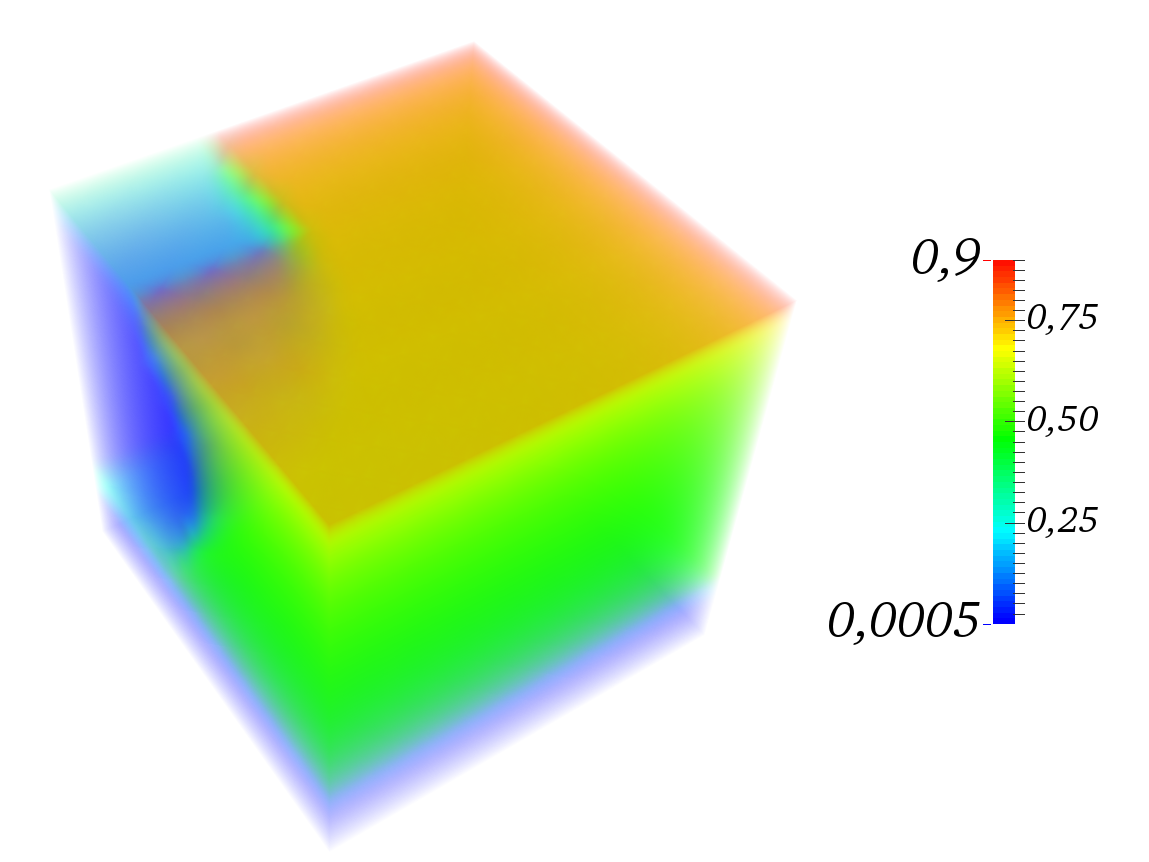
\includegraphics[width=1\textwidth]{test4/sg_200.png}
       \vspace{1cm}
       \caption{Насыщенность $S_g$ в момент времени $t=200$с}
    \end{minipage}
    \hfill
    \begin{minipage}[h]{0.49\textwidth}
       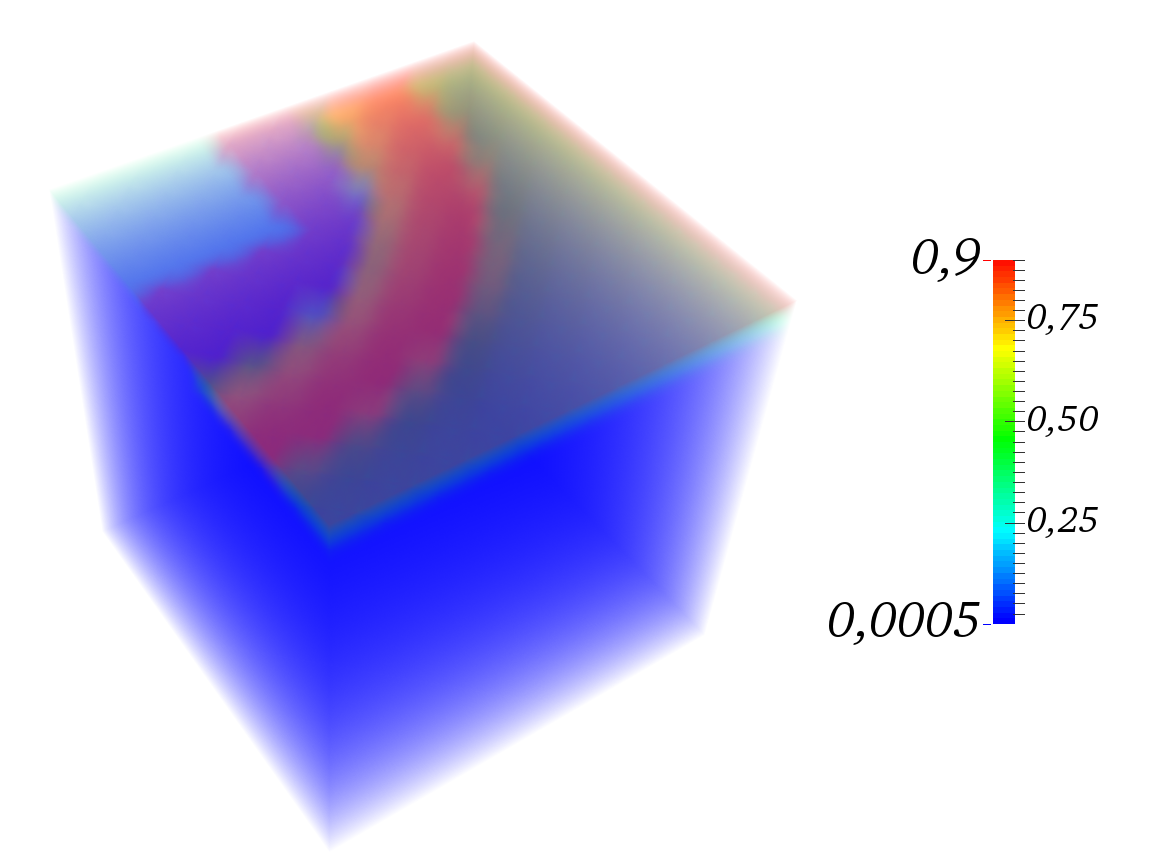
\includegraphics[width=1\textwidth]{test4/sg_1000.png}
       \vspace{1cm}
       \caption{Насыщенность $S_g$ в момент времени $t=1000$с}
    \end{minipage}
    \vspace{3cm}
    \vfill
    \begin{minipage}[h]{0.49\textwidth}
       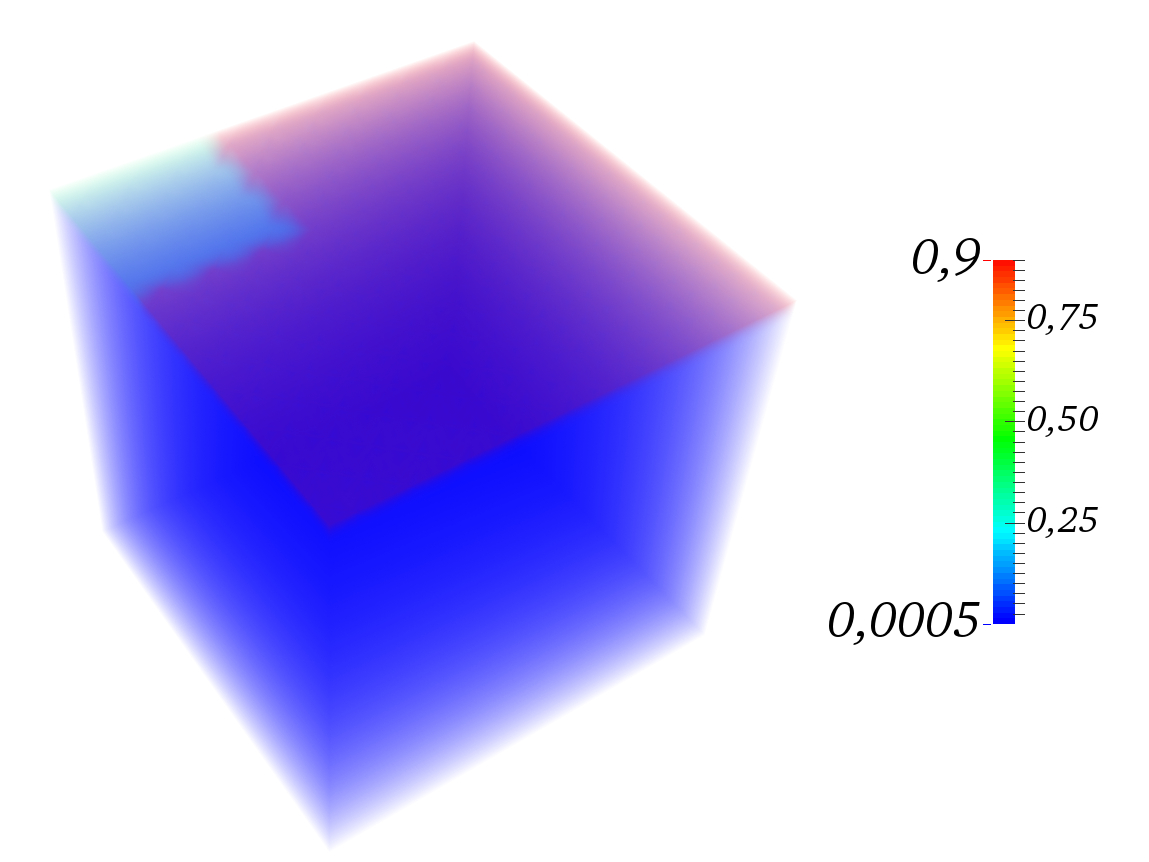
\includegraphics[width=1\textwidth]{test4/sg_2000.png}
       \vspace{1cm}
       \caption{Насыщенность $S_g$ в момент времени $t=2000$с}
    \end{minipage}
    \hfill
    \begin{minipage}[h]{0.49\textwidth}
       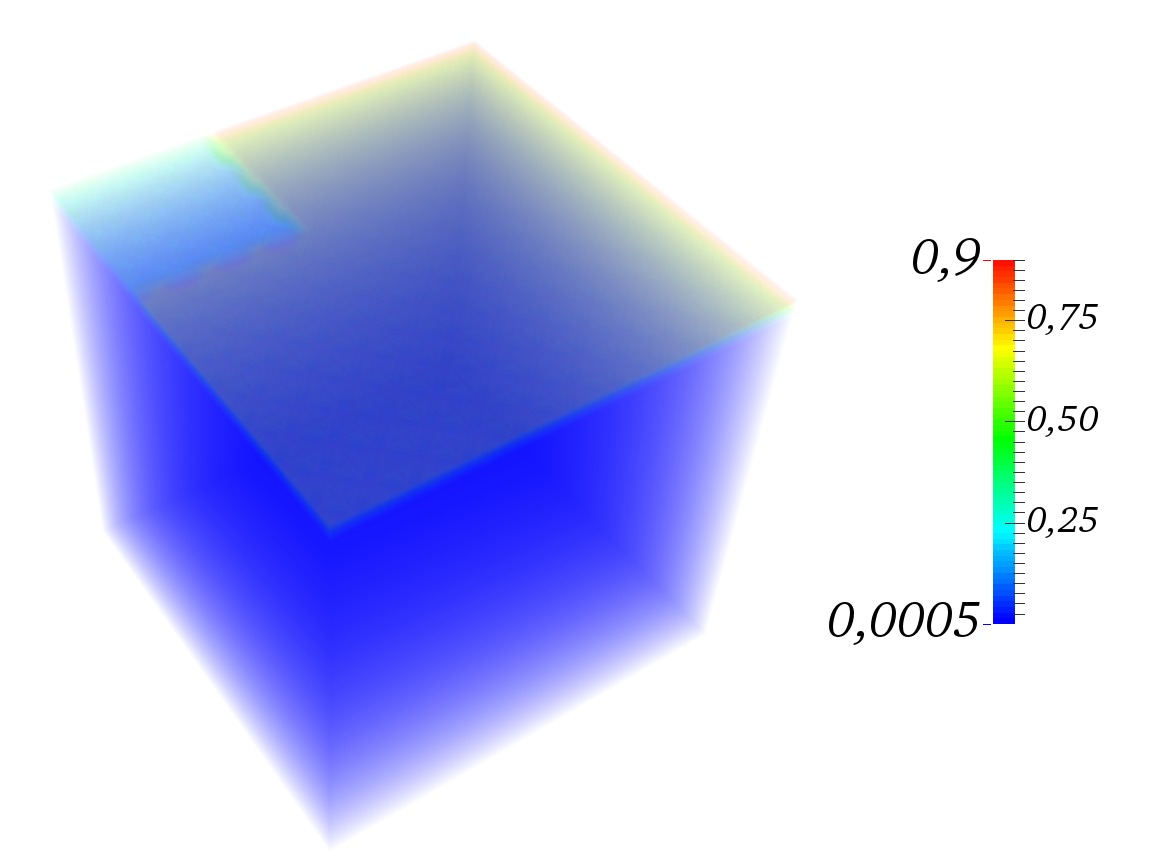
\includegraphics[width=1\textwidth]{test4/sg_6600.png}
       \vspace{1cm}
       \caption{Насыщенность $S_g$ в момент времени $t=6600$с}
       \label{t4_pic_end}
    \end{minipage}
    \hfill  
  \end{center}
\end{figure}
